%\title{Article HW Template}

\documentclass[12pt]{article}
\usepackage[paper=a4paper,top=1in, bottom=1in, right=1in, left=.7in]{geometry}
\usepackage{amsthm, amssymb, amsfonts, amsmath}
\usepackage{graphicx}
\usepackage{tikz}
\usetikzlibrary{calc,shapes}
\usepackage{enumitem}
\usepackage{mathtools}
\usepackage{mathrsfs}
\usepackage{tikz-cd}
\usepackage{hyperref, mathabx}
\usepackage{algorithm}
\usepackage{algpseudocode}
\renewcommand{\algorithmicrequire}{\textbf{Input:}}
\renewcommand{\algorithmicensure}{\textbf{Output:}}

\newcommand{\boxitem}[2]{\vspace{.55cm}
	\item[#1]
	\leavevmode
	\strut
	\vadjust{%%
		\noindent
		\raisebox{\dimexpr\dp\strutbox+\ht\strutbox+1ex}[0pt][0pt]{\tikzmark{bl}}}%%
	#2
	
	\leavevmode
	\vadjust{%
		\noindent
		\hspace*{\dimexpr\textwidth+1ex}\tikzmark{br}}%%
	
	\tikz[overlay,remember picture]{\draw[black]
		(bl) rectangle
		(br);}}

\newcommand{\tikzmark}[1]{\tikz[overlay,remember picture] \node (#1) {};}

\newcommand{\R}{\mathbb{R}}
\newcommand{\Q}{\mathbb{Q}}
\newcommand{\Z}{\mathbb{Z}}
\newcommand{\N}{\mathbb{N}}
\newcommand{\p}{\mathbb{P}}
\newcommand{\E}{\mathbb{E}}
\newtheorem*{lemma}{Lemma}
\newtheorem{llemma}{Lemma}
\newtheorem*{theorem}{Theorem}
\newtheorem*{prop}{Proposition}

\begin{document}
	\null\hfill\begin{tabular}[t]{r@{}}
		Nikolas Mavrogeneiadis - 161014\\
		gravitorious \\
		University Of West Attica \\
		Department of Informatics and Computer Engineering\\
		Professor: Panagiotis Rouvelas\\
		\today
	\end{tabular}
	\\
	\centerline{\scshape{Graph Theory-Exercise Set 2}}
	
	\begin{enumerate}[listparindent=1.5em,
		parsep = 0pt]
		
	\boxitem{1.}{
		Which graphs have a diameter equal to 1?
	}
		\underline{Proof:} All complete graphs have a diameter equal to 1 because every pair of vertices are adjacent.
		
	\boxitem{2.}{
		If every degree vertex of a simple graph is greater than one, the graph $G$ contains a cycle.
	}
	\underline{Proof:} Suppose that the graph doesn't contain a cycle. Consider one path $P=(v_{0}, v_{1}, ..., v_{k})$ from $G$ with the maximum length. We know that the vertex $v_{k}$ is incident with at least one edge $e$ that hasn't been used from the path. If this edge $e$ is also incident with one vertex from path $P$, then $G$ has a cycle (which is a contradiction). If $e$ is incident with one vertex that doesn't belong to path $P$, then $P$ isn't the path with the maximum length, which again is a contradiction. So $G$ has a cycle.
	
	\boxitem{3.}{
		Find all $n$ such that $K_{n}$ is Eulerian.
	}
	\underline{Proof:} To be $K_{n}$ Eulerian, $n$ must be odd because if it isn't, every vertex degree is odd and can't be Eulerian. If n is odd, then every vertex degree is even and so contains an Eulerian circuit and $K_{n}$ is Eulerian.
	
	\boxitem{4.}{
		Let $G$ be a simple graph. Prove that:
		\\$i)$ If $G$ is Eulerian, then $L(G)$ is Eulerian.
		\\$ii)$ If $L(G)$ is Eulerian, then we can't conclude that $G$ is Eulerian.
	}
	\underline{Proof:} $i)$ We know that each vertex degree of $G$ is even number. From the definition of line graph we can deduce that for edge $e(v,u) \in E(G)$ that becomes a vertex in $L(G)$, it has degree $deg(v)-1+deg(u)-1$ that it is also an even number. So $L(G)$ is Eulerian. \\
	$ii)$ If $L(G)$ is Eulerian this means that each vertex degree of $L(G)$ is even number. This vertex will become an edge $e(v,u)$ on $G$ with $deg(v)+deg(u) = even$. In this case, we can't deduce whether $deg(v)$ and $deg(u)$ are even or not. This completes the proof.
	
	\newpage
	
	\boxitem{6.}{
		Find a Hamiltonian graph that its closure is not complete.
	}
	\underline{Proof:}
	\begin{figure}[h]
		\centering
		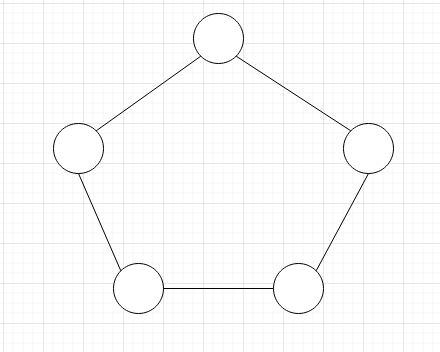
\includegraphics[width=0.55\textwidth]{pic1}
		\caption{Hamiltonian graph that its closure is a complete graph}
		\label{fig:mesh1}
	\end{figure}\\

	\boxitem{7.}{
		If simple graph $G$ is Eulerian, then $L(G)$ is Hamiltonian.
	}
	\underline{Proof:}
	Because $G$ is Eulerian this means that exists an Eulerian circuit. Let the edges of this circuit be $(e_{1}, e_{2}, ..., e_{n})$. Of course $e_{1}$ and $e_{n}$ has a common vertex $v_{n} \in V(G)$. We can easily construct a Hamiltonian cycle on $L(G)$ by replacing two incident edges with the common vertex. This means that the cycle $(v_{12}, v_{23}, ..., v_{n-1n})$ is a Hamiltonian cycle.
	
	\boxitem{9.}{
		Give an $O(|V|+|E|)$ algorithm that takes as input a graph $G=(V,E)$ and one edge $e$ and checks if this edge is bridge.
	}
	
	\underline{Proof:} Create a graph without this edge and run DFS algorithm counting the vertices that are visited (let $x$). If $x=|V|$ then e is not bridge, else is bridge. 
	
	\end{enumerate}
\end{document}
